%% Преамбула TeX-файла

% 1. Стиль и язык
\documentclass[utf8x, 12pt]{G7-32} % Стиль (по умолчанию будет 14pt)

% Остальные стандартные настройки убраны в preamble.inc.tex.
\sloppy

% Настройки стиля ГОСТ 7-32
% Для начала определяем, хотим мы или нет, чтобы рисунки и таблицы нумеровались в пределах раздела, или нам нужна сквозная нумерация.
\EqInChapter % формулы будут нумероваться в пределах раздела
\TableInChapter % таблицы будут нумероваться в пределах раздела
\PicInChapter % рисунки будут нумероваться в пределах раздела
\usepackage{slashbox}

% Добавляем гипертекстовое оглавление в PDF
\usepackage[
bookmarks=true, colorlinks=true, unicode=true,
urlcolor=black,linkcolor=black, anchorcolor=black,
citecolor=black, menucolor=black, filecolor=black,
]{hyperref}

% Изменение начертания шрифта --- после чего выглядит таймсоподобно.
% apt-get install scalable-cyrfonts-tex

\IfFileExists{cyrtimes.sty}
    {
        \usepackage{cyrtimespatched}
    }
    {
        % А если Times нету, то будет CM...
    }

\usepackage{graphicx}   % Пакет для включения рисунков

% С такими оно полями оно работает по-умолчанию:
% \RequirePackage[left=20mm,right=10mm,top=20mm,bottom=20mm,headsep=0pt]{geometry}
% Если вас тошнит от поля в 10мм --- увеличивайте до 20-ти, ну и про переплёт не забывайте:
\geometry{right=20mm}
\geometry{left=30mm}


% Пакет Tikz
\usepackage{tikz}
\usetikzlibrary{arrows,positioning,shadows}

% Произвольная нумерация списков.
\usepackage{enumerate}

% ячейки в несколько строчек
\usepackage{multirow}

% itemize внутри tabular
\usepackage{paralist,array}

% Центрирование подписей к плавающим окружениям
\usepackage[justification=centering]{caption}


% Настройки листингов.
\ifPDFTeX
% 8 Листинги

\usepackage{listings}
\usepackage{wrapfig}
% Значения по умолчанию
\lstset{
  basicstyle= \footnotesize,
  breakatwhitespace=true,% разрыв строк только на whitespacce
  breaklines=true,       % переносить длинные строки
%   captionpos=b,          % подписи снизу -- вроде не надо
  inputencoding=koi8-r,
  numbers=left,          % нумерация слева
  numberstyle=\footnotesize,
  showspaces=false,      % показывать пробелы подчеркиваниями -- идиотизм 70-х годов
  showstringspaces=false,
  showtabs=false,        % и табы тоже
  stepnumber=1,
  tabsize=4,              % кому нужны табы по 8 символов?
  frame=single
}

% Стиль для псевдокода: строчки обычно короткие, поэтому размер шрифта побольше
\lstdefinestyle{pseudocode}{
  basicstyle=\small,
  keywordstyle=\color{black}\bfseries\underbar,
  language=Pseudocode,
  numberstyle=\footnotesize,
  commentstyle=\footnotesize\it
}

% Стиль для обычного кода: маленький шрифт
\lstdefinestyle{realcode}{
  basicstyle=\scriptsize,
  numberstyle=\footnotesize
}

% Стиль для коротких кусков обычного кода: средний шрифт
\lstdefinestyle{simplecode}{
  basicstyle=\footnotesize,
  numberstyle=\footnotesize
}

% Стиль для BNF
\lstdefinestyle{grammar}{
  basicstyle=\footnotesize,
  numberstyle=\footnotesize,
  stringstyle=\bfseries\ttfamily,
  language=BNF
}

% Определим свой язык для написания псевдокодов на основе Python
\lstdefinelanguage[]{Pseudocode}[]{Python}{
  morekeywords={each,empty,wait,do},% ключевые слова добавлять сюда
  morecomment=[s]{\{}{\}},% комменты {а-ля Pascal} смотрятся нагляднее
  literate=% а сюда добавлять операторы, которые хотите отображать как мат. символы
    {->}{\ensuremath{$\rightarrow$}~}2%
    {<-}{\ensuremath{$\leftarrow$}~}2%
    {:=}{\ensuremath{$\leftarrow$}~}2%
    {<--}{\ensuremath{$\Longleftarrow$}~}2%
}[keywords,comments]

% Свой язык для задания грамматик в BNF
\lstdefinelanguage[]{BNF}[]{}{
  morekeywords={},
  morecomment=[s]{@}{@},
  morestring=[b]",%
  literate=%
    {->}{\ensuremath{$\rightarrow$}~}2%
    {*}{\ensuremath{$^*$}~}2%
    {+}{\ensuremath{$^+$}~}2%
    {|}{\ensuremath{$|$}~}2%
}[keywords,comments,strings]

% Подписи к листингам на русском языке.
\renewcommand\lstlistingname{\cyr\CYRL\cyri\cyrs\cyrt\cyri\cyrn\cyrg}
\renewcommand\lstlistlistingname{\cyr\CYRL\cyri\cyrs\cyrt\cyri\cyrn\cyrg\cyri}

\else
\usepackage{local-minted}
\fi
\usepackage{dirtytalk}
\usepackage{algorithm2e}
\usepackage[noend]{algpseudocode}
\usepackage{csquotes}
\usepackage[at]{easylist}
\usepackage{pgfplots}
\usepackage{listings}
\usepackage{listings-golang}

% Полезные макросы листингов.
% Любимые команды
\newcommand{\Code}[1]{\textbf{#1}}


\begin{document}

\frontmatter % выключает нумерацию ВСЕГО; здесь начинаются ненумерованные главы: реферат, введение, глоссарий, сокращения и прочее.

% Команды \breakingbeforechapters и \nonbreakingbeforechapters
% управляют разрывом страницы перед главами.
% По-умолчанию страница разрывается.

% \nobreakingbeforechapters
% \breakingbeforechapters

% НАЧАЛО ТИТУЛЬНОГО ЛИСТА
\begin{center}
	\hfill \break
	\textit{
		\normalsize{Государственное образовательное учреждение высшего профессионального образования}}\\ 
	
	\textit{
		\normalsize  {\bf  «Московский государственный технический университет}\\ 
		\normalsize  {\bf имени Н. Э. Баумана»}\\
		\normalsize  {\bf (МГТУ им. Н.Э. Баумана)}\\
	}
	\noindent\rule{\textwidth}{2pt}
	\hfill \break
	\noindent
	\\
	\noindent
	\\
	\hfill\break
	\hfill \break
	\hfill \break
	\hfill \break
	
	\hfill \break
	\large{Лабораторная работа №3\\ \textquote{Сортировки}}\\
	\hfill \break
	\hfill \break
	\hfill \break
	\hfill \break
	\hfill \break	
	\normalsize {
		\begin{minipage}[t]{7cm}
		\end{minipage}
		\hfill
		\begin{minipage}[t]{7cm}
			\flushright
			Студент: Камакин А.С.\\
			Группа: ИУ7-53\\
			Преподаватель: Волкова Л.Л.
		\end{minipage}
	}\\
	\hfill \break	
	\hfill \break
	\hfill \break
	\hfill \break
	\hfill \break
\end{center}
\hfill \break
\hfill \break
\begin{center} Москва 2017 \end{center}

\thispagestyle{empty} % 
% КОНЕЦ ТИТУЛЬНОГО ЛИСТА

\newpage
% \tableofcontents

\mainmatter % это включает нумерацию глав и секций в документе ниже

\paragraph{Системные характеристики и окружение}
\begin{itemize}
	\item Операционная система: Ubuntu 17.10 64-bit
	\item Память: 15,4 GiB
	\item Процессор: Intel® Core™ i5-3320M CPU @ 2.60GHz × 4
\end{itemize}

Пояснение: Стандартная системная утилита показывает, что в системе 4 ядра, но не говорит какие именно. Чтобы точно узнать количество ядер необходимо выполнить одну и следующих команд: cat /proc/cpuinfo | grep 'core id' или lscpu (поле Core(s) per socket)
\\

Пример выполнения команды cat /proc/cpuinfo | grep 'core id':\\
core id		: 0\\
core id		: 0\\
core id		: 1\\
core id		: 1\\

Пример выполнения команды lscpu:\\
CPU op-mode(s):      32-bit, 64-bit\\
Byte Order:          Little Endian\\
CPU(s):              4\\
On-line CPU(s) list: 0-3\\
Thread(s) per core:  2\\
Core(s) per socket:  2\\
Socket(s):           1\\
NUMA node(s):        1\\
Vendor ID:           GenuineIntel\\
CPU family:          6\\
Model:               58\\
Model name:          Intel(R) Core(TM) i5-3320M CPU @ 2.60GHz\\
Stepping:            9\\
CPU MHz:             2594.117\\
CPU max MHz:         3300,0000\\
CPU min MHz:         1200,0000\\
BogoMIPS:            5188.23\\
Virtualization:      VT-x\\

Можно сделать вывод, что у тестируемой среды есть 2 реальных и 4 логических ядра, что достигается за счет технологии hyperthreading.

\newpage

\paragraph{Терминология}
\\
Бенчмарк - эталонный тест производительности компьютерной системы.\\
gobench - инструмент для проведения бенчмарков в языке Go.\\
Горутина (goroutine) - легковесный поток.\\
\\
Отличия горутины от потока:

\begin{itemize}
	\item Можно запустить больше горутин на ОС чем потоков
	\item У горутин динамически растущий по мере необходимости сегментный стек
	\item Время старта горутины меньше чем у потока
	\item Горутины поставляются с механизмом безопасного общения - каналами
	\item Горутины позволяют избежать мьютекса для предоставления доступа к ресурсам
	\item Горутины мультиплексируются на небольшое количество потоков ОС, а не на отображение 1:1.
\end{itemize}

\newpage

\paragraph{Функция слияния общая для всех алгоритмов}
\begin{center}
	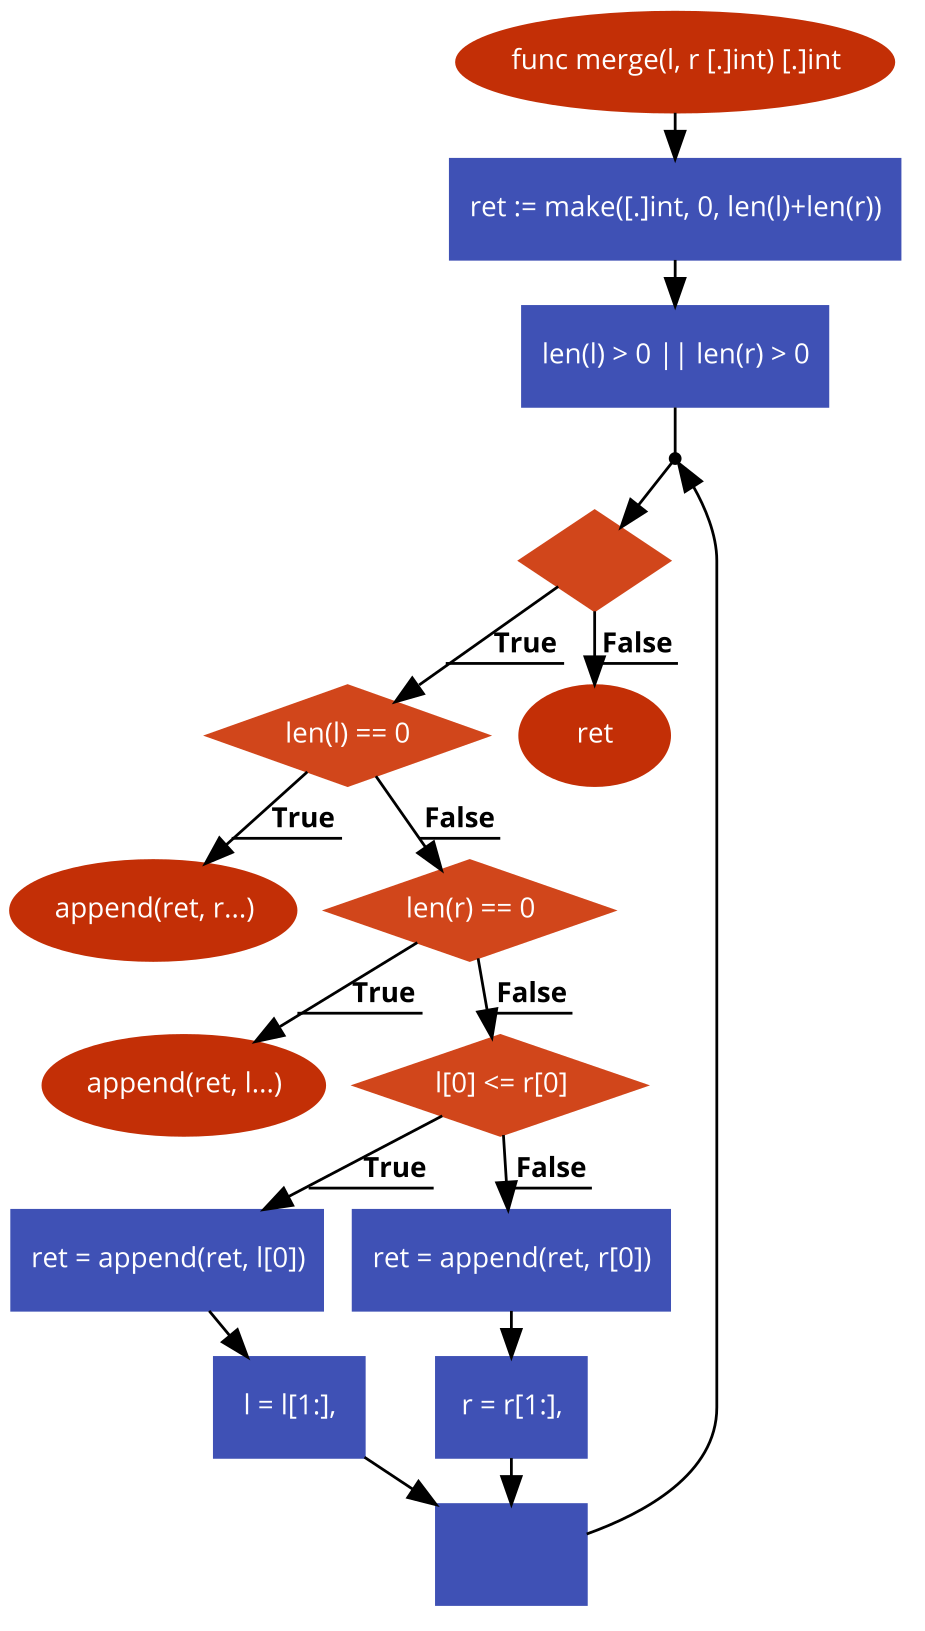
\includegraphics[scale=0.32]{images/merge.png}
\end{center}

\newpage

\paragraph{Классическая сортировка слиянием}
\begin{center}
	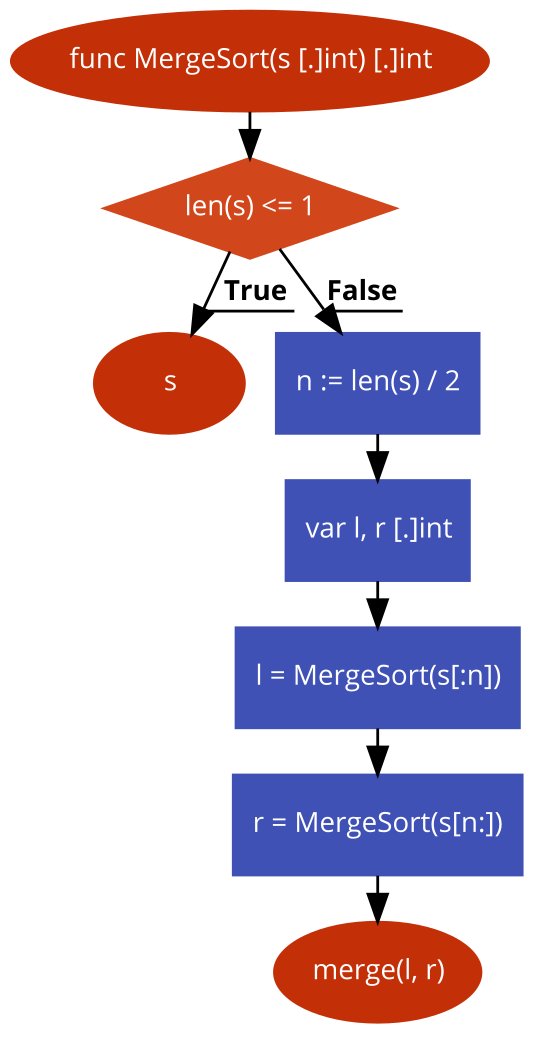
\includegraphics[scale=0.32]{images/mergeSort.png}
\end{center}

\newpage

\paragraph{Параллельная сортировка слиянием}
\begin{center}
	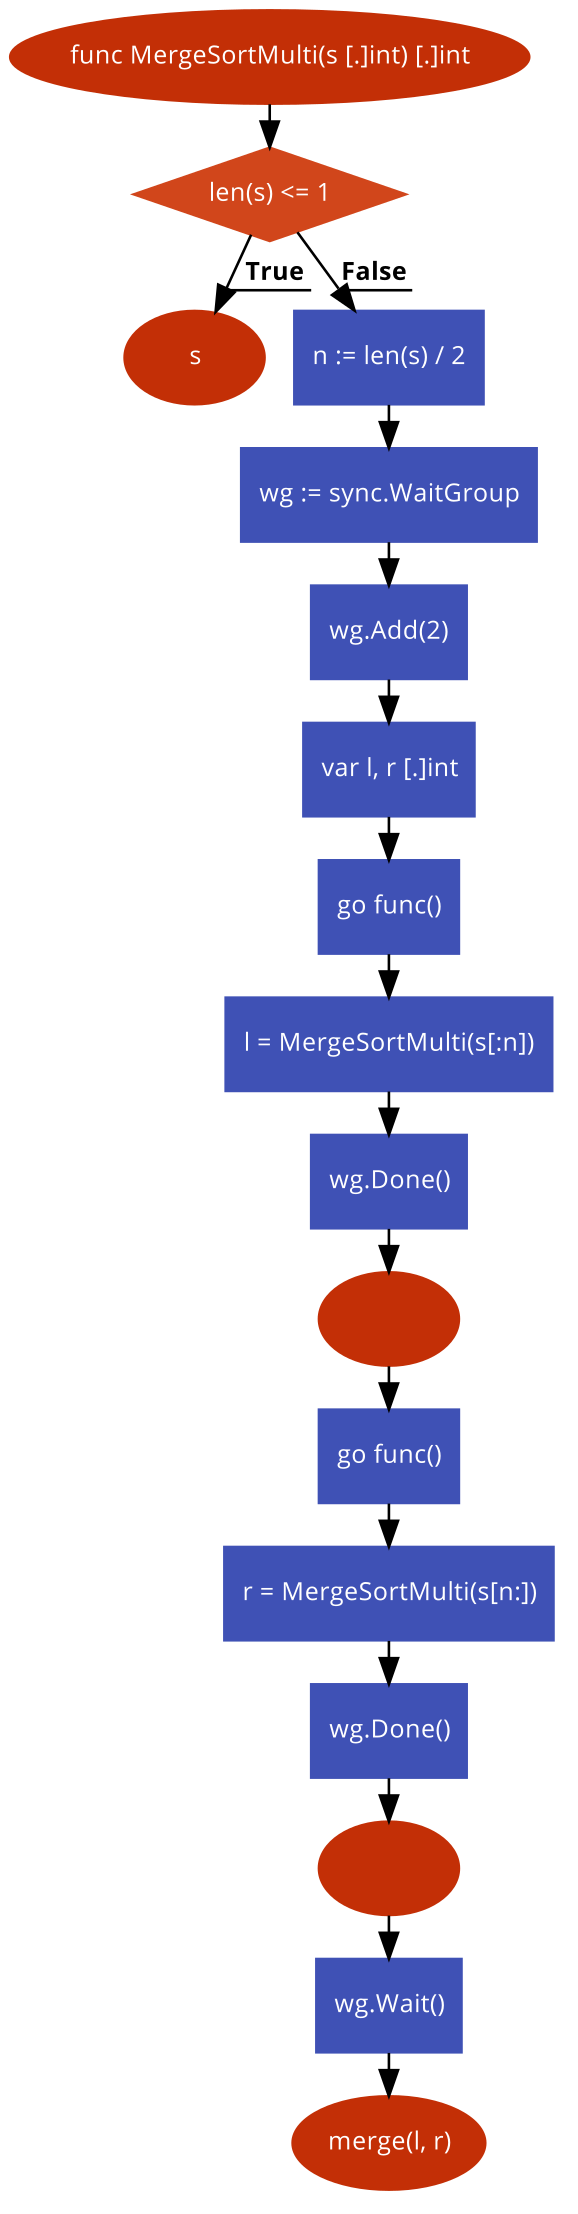
\includegraphics[scale=0.32]{images/mergeSortMulti.png}
\end{center}

\newpage

\paragraph{Комбинированная сортировка слиянием}
\begin{center}
	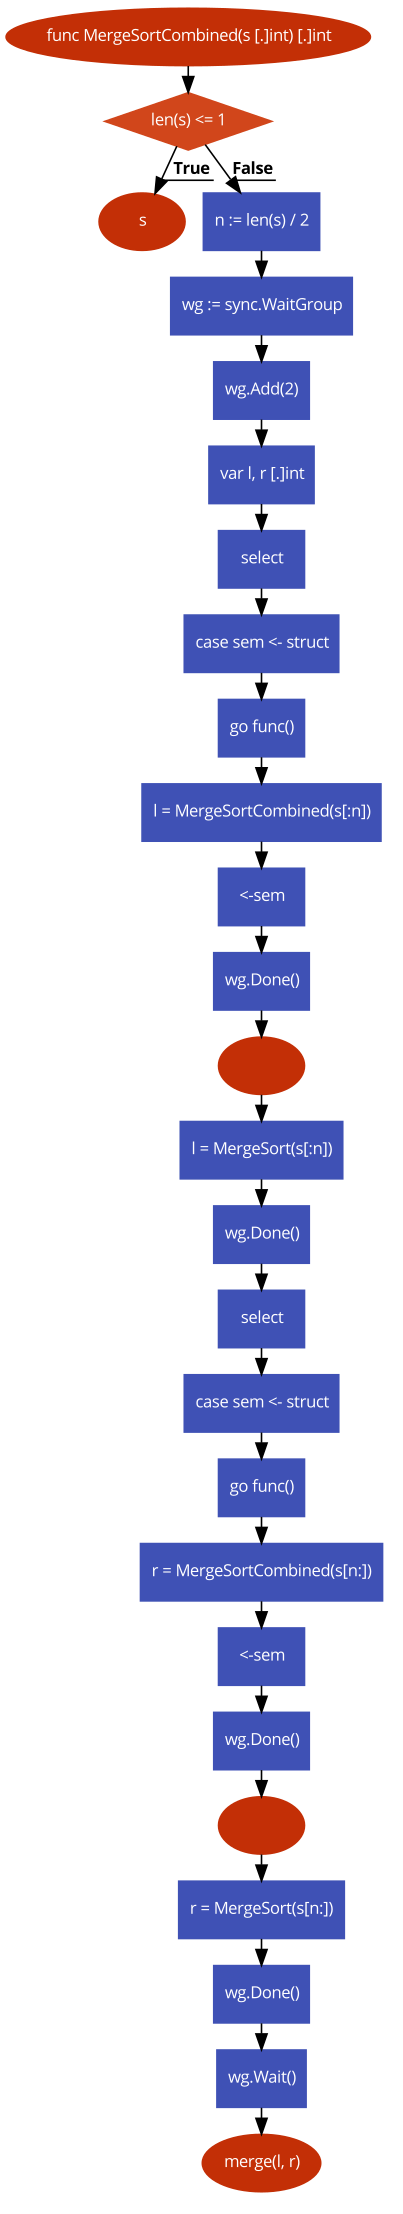
\includegraphics[scale=0.32]{images/mergeSortCombined.png}
\end{center}

\newpage

\paragraph{Графики}
\begin{center}
	\begin{tikzpicture}[yscale=0.8]
	\begin{axis}[
	title={Сравнение работы алгоритмов по времени (sorted, gobench)},
	xmode = log,
	log basis x=10,
	xlabel={длина строки $l$},
	ylabel={время $t(ns)$},
	xmin=0, xmax=101000,
	ymin=0, ymax=17000000,
	xtick={0,10,100,1000,10000,100000},%1000000},
	ytick={0,5000000,10000000,15000000},
	legend pos=north west,
	ymajorgrids=true,
	grid style=dashed,
	legend style={at={(0.5,-0.1)},anchor=north},
	]
	
	\addplot[
	color=red,
	mark=square,
	]
	coordinates {
		(10,659)(100,9098)(1000,102652)(10000,1265028)(100000,13886742)%(1000000,116267374)
	};
	\addlegendentry{Классическая}
	
	\addplot[
	color=blue,
	mark=square,
	]
	coordinates {
		(10,11937)(100,106255)(1000,579249)(10000,9888072)(100000,101543324)%(1000000,1192577864)
	};
	\addlegendentry{Параллельная}
	
	\addplot[
	color=green,
	mark=square,
	]
	coordinates {
		(10,9872)(100,114392)(1000,270951)(10000,1531330)(100000,11532055)%(1000000,87818725)
	};
	\addlegendentry{Комбинированная}
	
	\end{axis}
	\end{tikzpicture}
\end{center}

\begin{center}
	\begin{tikzpicture}[yscale=0.8]
	\begin{axis}[
	title={Сравнение работы алгоритмов по времени (random, gobench)},
	xmode = log,
	log basis x=10,
	xlabel={длина строки $l$},
	ylabel={время $t(ns)$},
	xmin=0, xmax=101000,
	ymin=0, ymax=17000000,
	xtick={0,10,100,1000,10000,100000},%1000000},
	ytick={0,5000000,10000000,15000000},
	legend pos=north west,
	ymajorgrids=true,
	grid style=dashed,
	legend style={at={(0.5,-0.1)},anchor=north},
	]
	
	\addplot[
	color=red,
	mark=square,
	]
	coordinates {
		(10,556)(100,9798)(1000,145247)(10000,1979934)(100000,21306925)%(1000000,233665988)
	};
	\addlegendentry{Классическая}
	
	\addplot[
	color=blue,
	mark=square,
	]
	coordinates {
		(10,8413)(100,98786)(1000,579853)(10000,10455389)(100000,114421901)%(1000000,1251387316)
	};
	\addlegendentry{Параллельная}
	
	\addplot[
	color=green,
	mark=square,
	]
	coordinates {
		(10,9546)(100,118593)(1000,285336)(10000,1911819)(100000,15256937)%(1000000,125206941)
	};
	\addlegendentry{Комбинированная}
	
	\end{axis}
	\end{tikzpicture}
\end{center}

\begin{center}
	\begin{tikzpicture}[yscale=0.8]
	\begin{axis}[
	title={Сравнение работы алгоритмов по времени (reversed, gobench)},
	xmode = log,
	log basis x=10,
	xlabel={длина строки $l$},
	ylabel={время $t(ns)$},
	xmin=0, xmax=101000,
	ymin=0, ymax=17000000,
	xtick={0,10,100,1000,10000,100000},%1000000},
	ytick={0,5000000,10000000,15000000},
	legend pos=north west,
	ymajorgrids=true,
	grid style=dashed,
	legend style={at={(0.5,-0.1)},anchor=north},
	]
	
	\addplot[
	color=red,
	mark=square,
	]
	coordinates {
		(10,544)(100,9065)(1000,113490)(10000,1402595)(100000,16016143)%(1000000,146387339)
	};
	\addlegendentry{Классическая}
	
	\addplot[
	color=blue,
	mark=square,
	]
	coordinates {
		(10,8374)(100,99514)(1000,556783)(10000,9502080)(100000,100411111)%(1000000,1242225349)
	};
	\addlegendentry{Параллельная}
	
	\addplot[
	color=green,
	mark=square,
	]
	coordinates {
		(10,9807)(100,113806)(1000,263942)(10000,1729743)(100000,12091641)%(1000000,93520440)
	};
	\addlegendentry{Комбинированная}
	
	\end{axis}
	\end{tikzpicture}
\end{center}

\newpage

\paragraph{Тестовые данные}\\

\begin{flushleft}
	\paragraph{Sorted}
\end{flushleft}

Время работы в наносекундах (ns):\\
\begin{tabular}{l*{6}{c}r}
	Алгоритм & 10 & 100 & 1000 & 10000 & 100000 & 1000000 \\
	\hline
	Классическая & 659 & 9098 & 102652 & 1265028 & 13886742 & 116267374 \\
	Параллельная & 11937 & 106255 & 579249 & 9888072 & 101543324 & 1192577864 \\
	Комбинированная & 9872 & 114392 & 270951 & 1531330 & 11532055 & 87818725 \\
\end{tabular}

\begin{flushleft}
	\paragraph{Random}
\end{flushleft}

Время работы в наносекундах (ns):\\
\begin{tabular}{l*{6}{c}r}
	Алгоритм & 10 & 100 & 1000 & 10000 & 100000 & 1000000 \\
	\hline
	Классическая & 556 & 9798 & 145247 & 1979934 & 21306925 & 233665988 \\
	Параллельная & 8413 & 98786 & 579853 & 10455389 & 114421901 & 1251387316 \\
	Комбинированная & 9546 & 118593 & 285336 & 1911819 & 15256937 & 125206941 \\
\end{tabular}

\begin{flushleft}
	\paragraph{Reversed}
\end{flushleft}

Время работы в наносекундах (ns):\\
\begin{tabular}{l*{6}{c}r}
	Алгоритм & 10 & 100 & 1000 & 10000 & 100000 & 1000000 \\
	\hline
	Классическая & 544 & 9065 & 113490 & 1402595 & 16016143 & 146387339 \\
	Параллельная & 8374 & 99514 & 556783 & 9502080 & 100411111 & 1242225349 \\
	Комбинированная & 9807 & 113806 & 263942 & 1729743 & 12091641 & 93520440 \\
\end{tabular}

\newpage

\paragraph{Оценка трудоемкостей алгоритмов}
\\
Примерная сложность функции $merge$: $1 + n(2 + 2 + 3 + 3 + 2) = 12n + 1 \simeq n$\\
Примерная cложность функции MergeSort: Функция будет вызываться пока $n$ не станет равным 1. Это можно представить в виде дерева растущего вниз, имеем, $2^h = n$, где $h$ - высота дерева, $n$ - количество элементов, отсюда следует $\log_2 n = h$\\
Общая сложность: $n * h = n * \log_2 n$

\begin{center}
	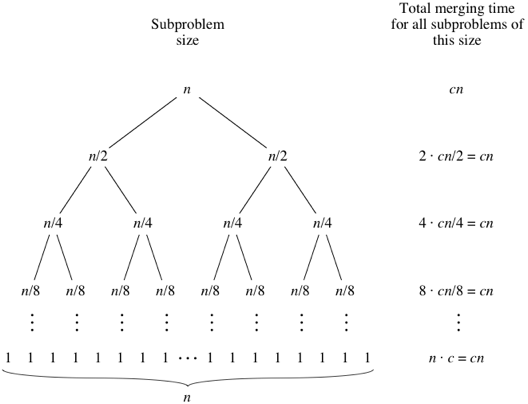
\includegraphics{images/mergeSortTree.png}
\end{center}

\begin{lstlisting}
func merge(l, r []int) []int {
	ret := make([]int, 0, len(l)+len(r))
	for len(l) > 0 || len(r) > 0 {
		if len(l) == 0 {
			return append(ret, r...)
		}
		if len(r) == 0 {
			return append(ret, l...)
		}
		if l[0] <= r[0] {
			ret = append(ret, l[0])
			l = l[1:]
		} else {
			ret = append(ret, r[0])
			r = r[1:]
		}
	}
	return ret
}

func MergeSort(s []int) []int {
	if len(s) <= 1 {
		return s
	}
	n := len(s) / 2
	var l, r []int
	l = MergeSort(s[:n])
	r = MergeSort(s[n:])
	return merge(l, r)
}
\end{lstlisting}

\paragraph{Заключение}

В ходе работы были описаны и реализованы различные варианты алгоритма сортировки слиянием (классический, параллельный и комбинированный), и был проведен сравнительный анализ их временной эффективности.

\backmatter %% Здесь заканчивается нумерованная часть документа и начинаются ссылки и
            %% заключение

\appendix   % Тут идут приложения

\end{document}

%%% Local Variables:
%%% mode: latex
%%% TeX-master: t
%%% End: